%----------------------------------------------------------------------------
\chapter{Case Study}\label{sect:case-study}
In this chapter I want to demonstrate the functionalities of Model-based test generation. For this I have created a sample system, which models a garage gate. First I describe the common functionality of this system, then I set-up the system requirements and finally I introduce the implementation and design decisions of the system for different model-based testing tools.

\section{System introduction}
The user can send action with the control switch to the control logic meaning that open or close the gate. If someone or something suddenly appears in the way of the gate, while it is moving, the movement stops. The motion sensor detects this interruption (the gate is blocked) or free status (the gate has free way). Before restarting the closing action, the control unit waits 5 seconds for the lighting warning. When the gate is finally closed, an additional sensor gives us plausibility for the gate physically closed state.

In this garage gate sample, we can have sensors, which measures the world around the system, and subsystems for realizing some logic in their functionalities.

This garage gate software system consists of 6 different units (see figure \figref{overalBDD}). These are the following: a gate, a lamp, a remote Controller, a control logic, motion sensor, a motor and a gate closed-state detection sensor.

The communication between the components is based on dedicated signal types like MotorSignal or LampSignal. These types mainly focusing on the control commands for each block.

The system consists 6 elements:
\begin{itemize}
	\item Lamp: This component is represents the lamp itself, which can be turn off or on.
	\item Motor: This block can move the gates to opened and closed state.
	\item MotionSensor: These sensors are on the two pillars of the gate, and detect if something has appeared between them.
	\item SwitchController: This block is for the remote controller realization. It has an \textit{open} and a \textit{close} button function.
	\item GateStateSensor: This sensor can detect if the gate is in the final closed or opened state, when physically the movement must be stopped.
	\item GarageGateLogic: This block implements the safety logic for the gate system, therefore it has all of the necessary information about the components.
\end{itemize}

\begin{figure}[!ht]
	\centering
	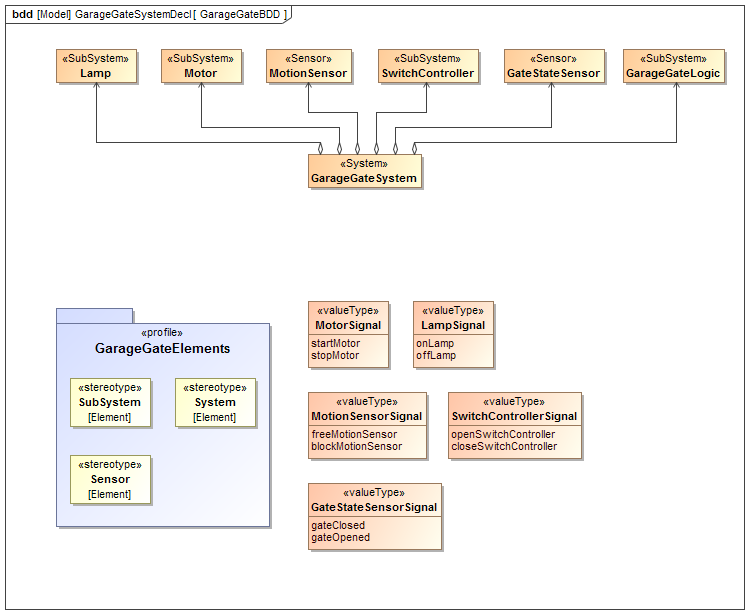
\includegraphics[width=100mm, keepaspectratio]{figures/magicDraw/bdd__GarageGateBDD.png}
	\caption{Garage system components and signals}
	\label{fig:overalBDD}
\end{figure}

\section{Software Requirements}\label{subsect:SW-REQ}
\subsection{Lamp}
\begin{description}
	\item [REQ-01-1] The lamp lighting frequency should be 1 second.
	\item [REQ-01-2] One lighting section is 5 seconds long.
	\item [REQ-01-3] The warning lighting must happen while the gate is closing, and the motion sensor gives free status after a blocked event.
\end{description}

\subsection{Motor}
\begin{description}
	\item [REQ-02-1] While the motor is running, the gate should get into the opposite state (opened/closed).
	\item [REQ-02-2] The motor moving operation can be stopped and resumed by the control logic.
%	\item [REQ-02-3] 
\end{description}

\subsection{Motion Sensor}
\begin{description}
	\item [REQ-03-1] The sensor must detect if anything is between the two pillars of the gate (so between the two sensors). 
	\item [REQ-03-2] If the sensor detects a movement, a \textit{blocking} signal must be sent immediately to the \textit{Control Logic}.
	\item [REQ-03-3] If the sensor can not detect any more the movement between the two gates, a \textit{free} signal must be sent to the \textit{Control Logic}.
	\item [REQ-03-4] When the sensor detects free status after the blocking status, there must be at least 3 seconds until the first \textit{free} signal can be sent to the \textit{Control Logic}.
\end{description}

\subsection{Switch Controller}
\begin{description}
	\item [REQ-04-1] The controller should have an \textit{open} and a \textit{close} gate action button.
	\item [REQ-04-2] One action must be completely finished to start a new action. 
\end{description}

\subsection{GateStateSensor}
\begin{description}
	\item [REQ-05-1] It must detect the final closed/opened state of the \textit{gate}, and send information about it to the \textit{Control Logic}.
	\item [REQ-05-2] In the final states the gate can not be moved forward.
\end{description}

\subsection{GarageGateLogic}
\begin{description}
	\item [REQ-06-1] The \textit{Control Logic} can get actions from the \textit{Switch Controller}. One action must be finished to receive new actions.
	\item [REQ-06-2] While the gates are moving (by an action from the \textit{Switch Controller}), the \textit{Control Logic} should stop the movement, if it gets a \textit{blocking} sign from the \textit{Motion Sensor} and stop the \textit{Motor}. Consequently the \textit{Control Logic} should continue the movement, if it gets a \textit{free} sign from the \textit{Motion Sensor} and start the \textit{Motor}.
	\item [REQ-06-3] The \textit{Control Logic} can receive the signals from the \textit{Motion Sensor}, \textit{Lamp}, \textit{Switch Controller} and \textit{Gate State Sensor}.
	\item [REQ-06-4] The \textit{Control Logic} must communicate to each component with dedicated signal types.
\end{description}

\section{System model representation}\label{subsect:Representation}
\paragraph{Communication between blocks}
In this section I want demonstrate the logical behaviour and communication constraints for the Garage Gate sample system.
The component communication is described with the following figure \figref{GateLogicComm}

\begin{figure}[!ht]
	\centering
	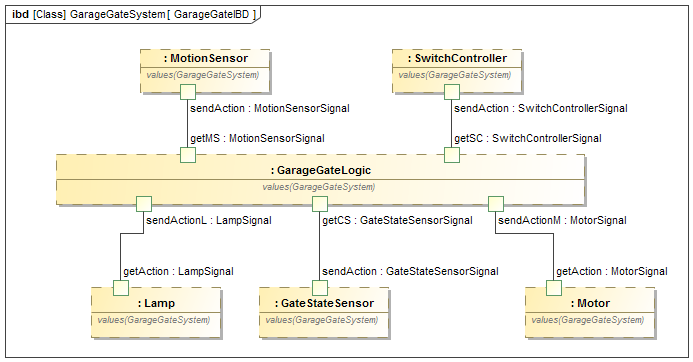
\includegraphics[width=150mm, keepaspectratio]{figures/magicDraw/ibd__GarageGateSystem__GarageGateIBD.png}
	\caption{Gate controller internal block diagram}
	\label{fig:GateLogicComm}
\end{figure}

The sensors and subsystems connects to the \textit{GarageGateLogic}, to its dedicated ports. Basically the \textit{SwitchController} ,\textit{MotionSensor} and \textit{GateStateSensor} sends control signals to the \textit{GarageGateLogic}, besides the \textit{Lamp} and \textit{Motor} components receives control signals from the \textit{GarageGateLogic}.

\paragraph{Logical operation}

The \figref{GateLogicComm} figure introduce the communication between the above listed blocks.

\begin{figure}[!ht]
	\centering
	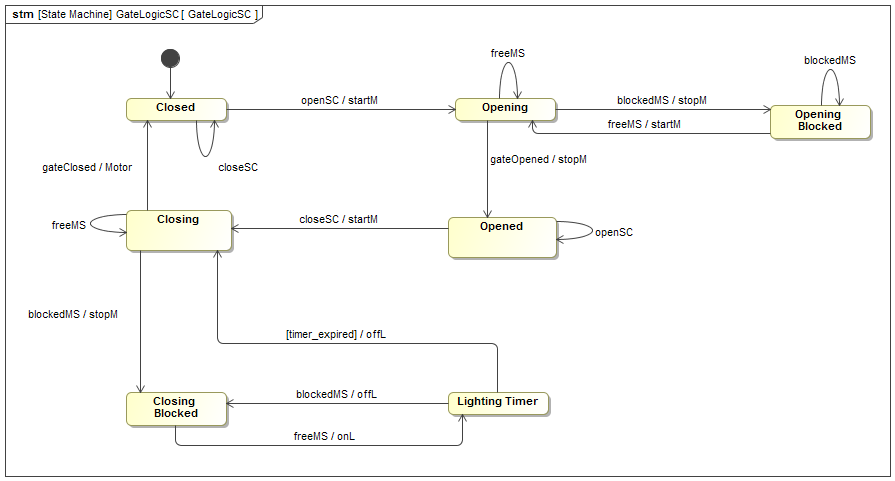
\includegraphics[width=150mm, keepaspectratio]{figures/magicDraw/GateLogicSC.png}
	\caption{Garage gate state machine diagram}
	\label{fig:Garage Statemachine}
\end{figure}

A garage gate fundamentally have 2 main states, the \textit{Opened} and \textit{Closed} states, which is shown below on \figref{Garage Statemachine} figure. First of all we can start from the initial \textit{Closed} state, where the \textit{Switch Controller} can open the gate with an 'open' command. This command sets the state machine in an \textit{Opening} state, while starting the motor functions. While opening the gate, somebody or something can move into the way of the gate, so this becomes \textit{Block Opening}. The gate is opening again, if the blocking object moved out of the way consequently it is free. After the \textit{Opening} phase succeeded the gate is \textit{Opened}. 

In this state we can 'close' the gate with a simple command by the \textit{Switch Controller}, and the state machine goes to the \textit{Closing} state. There could be also a blocking action, which stops the closing movement. From this state the gate is starting the closing movement again after a few seconds \textit{Lighting}. When the closing action finished the gate is \textit{Closed} and the motor has been stopped.


%TODO define what testing scenarios i will use
\paragraph{Testing goals}
I have decided to test the proper functionality of the whole garage gate system. Therefore the test scenario is to achieve all states in the state-machine model and to test most of the transitions from that.

